%% Paper B — verification timing under replay uncertainty.  Development
%% template: the ICML 2026 style kit (icml2026.sty / icml2026.bst); swap in the
%% official ICML 2027 kit when it is published.  Double-blind while the package
%% is loaded without [accepted]/[preprint].
%%
%% Research-draft status: sections contain PLANNED results only.  No fabricated
%% curves or performance numbers.  Build:  make pdf  (from papers/paper_b/).

\documentclass{article}
\usepackage[T1]{fontenc}
\usepackage[utf8]{inputenc}
\usepackage{microtype}
\usepackage{graphicx}
\usepackage{booktabs}
\usepackage{hyperref}
\usepackage{icml2026}
\usepackage{amsmath,amssymb,mathtools}
\usepackage{amsthm}
\usepackage{float}
\usepackage{enumitem}
\usepackage{xcolor}
\usepackage{tikz}
\usetikzlibrary{arrows.meta,fit,positioning,shapes.geometric}
\usepackage[capitalize,noabbrev]{cleveref}

\hypersetup{
  colorlinks=true,
  linkcolor=blue!50!black,
  citecolor=blue!50!black,
  urlcolor=blue!50!black
}

\newcommand{\Gset}{\mathcal{G}}
\newcommand{\Dcal}{\mathcal{D}}
\newcommand{\E}{\mathbb{E}}
\newcommand{\Prb}{\mathbb{P}}
\DeclareMathOperator*{\argmax}{arg\,max}

\theoremstyle{plain}
\newtheorem{theorem}{Theorem}
\newtheorem{proposition}[theorem]{Proposition}
\newtheorem{lemma}[theorem]{Lemma}
\newtheorem{corollary}[theorem]{Corollary}
\theoremstyle{definition}
\newtheorem{definition}[theorem]{Definition}
\newtheorem{assumption}[theorem]{Assumption}
\newtheorem{example}[theorem]{Example}
\theoremstyle{remark}
\newtheorem{remark}[theorem]{Remark}

\crefname{theorem}{Theorem}{Theorems}
\Crefname{theorem}{Theorem}{Theorems}
\crefname{proposition}{Proposition}{Propositions}
\Crefname{proposition}{Proposition}{Propositions}
\crefname{lemma}{Lemma}{Lemmas}
\Crefname{lemma}{Lemma}{Lemmas}
\crefname{corollary}{Corollary}{Corollaries}
\Crefname{corollary}{Corollary}{Corollaries}
\crefname{definition}{Definition}{Definitions}
\Crefname{definition}{Definition}{Definitions}
\crefname{assumption}{Assumption}{Assumptions}
\Crefname{assumption}{Assumption}{Assumptions}
\crefname{example}{Example}{Examples}
\Crefname{example}{Example}{Examples}
\crefname{remark}{Remark}{Remarks}
\Crefname{remark}{Remark}{Remarks}

\icmltitlerunning{When to Spend a Verification Budget under Replay Uncertainty}

\begin{document}

\twocolumn[
  \icmltitle{When to Spend a Verification Budget under Replay Uncertainty}

  \begin{icmlauthorlist}
    \icmlauthor{Anonymous Authors}{anon}
  \end{icmlauthorlist}
  \icmlaffiliation{anon}{Anonymous Affiliation, Anonymous City, Anonymous Country}
  \icmlcorrespondingauthor{Anonymous Authors}{anonymous@example.org}

  \icmlkeywords{verification timing, agent oversight, replay uncertainty,
    budgeted decision making, sequential control}

  \vskip 0.3in
]

% The development style prints an ICML under-review notice by default.  This
% paper is a research draft, not a submission, so the notice is replaced with
% the honest status.  It must be redefined before the notice is printed.
\makeatletter
\renewcommand{\Notice@String}{Research draft: results are planned; no experimental claims.}
\makeatother

\printAffiliationsAndNotice{}

\begin{abstract}
Verification can improve an agent's result, consume resources without benefit,
or remove a more valuable opportunity to check later.  We study a fixed
verification-and-response regime with at most one use across two online
checkpoints.  A paired branch-tree design compares verifying now, reserving
verification for later, and never verifying on the original root population,
including early termination and infeasibility.  Policy assessment separates
sampling uncertainty from an explicitly conditional allowance for
outcome-relevant reconstruction error.  The planned evaluation tests whether
preserving a later verification opportunity improves bounded task utility
against a matched repeated-myopic controller and a context-dependent VOI
scheduler at the same allowed
verifier and total-work budgets, and whether conclusions survive plausible
reconstruction error.  No live benefit or safety result is claimed before this
evaluation: every quantitative statement in this draft is \emph{planned}.

\end{abstract}

\section{Introduction}
\label{sec:b-introduction}

An autonomous experimentation agent that can call a verifier faces a timing
question before it faces a ranking question.  A verification budget spent at an
early checkpoint may repair a candidate that the frozen continuation would have
carried to failure; the same budget spent at a later checkpoint may act on
information that does not exist yet.  Spending early can therefore improve a
result, consume resources without benefit, or remove a more valuable later
opportunity \citep{calibrationnotcontrol2026,harnessr12026}.  This paper studies
the timing question directly for a fixed verification-and-response regime that
may be used \emph{at most once} across two online checkpoints.

\paragraph{Problem.}
Along each \emph{original root} (one independent run of the frozen agent from a
task template) two online checkpoints are eligible.  A controller may spend its
single verification at checkpoint 1, reserve it and spend it at checkpoint 2 if
that checkpoint is reached, or never verify.  Early termination and
infeasibility are part of the problem: a root that ends before checkpoint 2, or
at which verification is unavailable, remains in the original-root population
and is analysed under its registered fallback.  The regime is fixed and frozen:
the verifier checks consistency against \emph{visible} development diagnostics,
and the response rule replaces a candidate only on a strict visible improvement,
leaving ties unchanged.  The hidden evaluation is never visible to the agent or
the verifier.

\paragraph{Primary hypothesis (N2).}
The frozen two-checkpoint controller improves the original-root mean utility $U$
against \emph{both} a repeated-myopic controller and a BAVAR-inspired
context-dependent VOI scheduler, at the same allowed verifier and total-work
budgets.  The two
primary contrasts are tested with simultaneous intervals, with template families
as the sampling units and a prespecified treatment of batch coupling
(\cref{sec:b-statistics}).  Decision rules follow the registered design: a
contrast is supported when its adjusted lower confidence bound exceeds zero; the
practical target is $0.02\,U$; a contrast whose adjusted upper bound is below
$0.02$ rejects the practical target; an interval spanning the target is
inconclusive, with no automatic budget expansion.

\paragraph{Validity constraint (N1).}
Policy assessment separates sampling uncertainty from an explicitly conditional
allowance for outcome-relevant reconstruction error.  Under a declared joint
discrepancy event of probability at most $p$, bounded utility, a fixed policy
and the required calibration independence, the population gain lower bound loses
at most $2p$; this is an application of the measurement bound of the anonymous
companion paper \citep{companion2026}, not a new safety theorem
(\cref{sec:b-theory}).  There is no
pointwise gate from a global $p$: a finite frozen policy family instead receives
simultaneous population lower bounds and abstains if none qualifies.  For the
two-checkpoint comparison the allowance is a joint path allowance $p_{\text{path}}$
covering the decision histories and the compared regime outcomes.

\paragraph{Falsifiers.}
N2 is falsified if the adjusted lower confidence bound does not exceed zero for
either primary comparator, or if the adjusted upper bound falls below the
$0.02$ practical target; an interval that spans the target is inconclusive.
N1's mathematical claim is falsified by a counterexample satisfying its stated
assumptions.  Its practical claim is falsified if adding the allowance does not
improve the declared utility/harm tradeoff at equal allowed resources, including
the always-abstain controller that satisfies validity while failing the
practical contribution.  Understated $p$ is a sensitivity failure, not a
refutation of the conditional proposition.

\paragraph{What this paper is not.}
It is not a claim that prediction and intervention value come apart; that is
prior work \citep{interventionparadox2026,calibrationnotcontrol2026}.  It is not
a new general identification theorem for replay; the measurement preconditions
are developed by the anonymous companion and assumed here as a contract.  It
does not claim the historical ordinal-sufficiency identity as its contribution;
with identical ridge features, penalties and rows the advantage learner and the
action-value difference are the same estimator, and that comparison is retained
only as an implementation equivalence check
(\cref{sec:b-theory,sec:b-equivalence}).  It reports no live result: every
performance number is marked \emph{planned}
(\cref{sec:b-experiments}).

\paragraph{Organisation.}
\Cref{sec:b-problem} states the two-checkpoint problem and the original-root
population.  \Cref{sec:b-regimes} fixes the three regimes on one tree.
\Cref{sec:b-data} gives the branch-record schema and the runtime qualification
boundary.  \Cref{sec:policy} defines the matched controllers and total-work
accounting.  \Cref{sec:b-theory} states the scoped population proposition and
the equivalence check.  \Cref{sec:b-experiments} is the planned evaluation with
the candidate-consistency task.  \Cref{sec:b-statistics} fixes outcomes,
allocation estimands and inference.  \Cref{sec:b-limitations} states
limitations, \cref{sec:related} positions the work at method level, and
\cref{sec:b-bridge} records the deferral of unrestricted sequential control.

\section{The two-checkpoint problem and the original-root population}
\label{sec:b-problem}

\paragraph{Budget-constrained dynamic algorithm configuration (DAC).}
We frame verification timing as configuring the executor agent's action at
two checkpoints. Two deviations from standard DAC delimit this framing.
First, instances are budget-coupled: the shared two-phase allocator enforces
$B=\lfloor qN\rfloor$ across a batch of original roots, rather than choosing
an unconstrained policy independently for each instance. Second, the horizon
and action set are minimal: two decision points, continue or verify, and at
most one verification per root. This is a bounded DAC instance, not a DAC
benchmark or a new RL method, and no optimality claim is made.

Full history is kept: $H_2$ contains $H_1$. No Markov guarantee is claimed
for a compressed representation. A compressed state needs a justified Markov
assumption; otherwise retain history or acknowledge partial observability.
Population estimation supplies neither that assumption nor a theorem that
learned timing beats tuned rules. Keep the current two-checkpoint problem
bounded; adaptive replay acquisition and more general dynamic algorithm
configuration are separate extensions, not completed contributions introduced
by a new citation.

\paragraph{Population and unit.}
The population is a distribution over \emph{template families}.  A template
family generates one or more \emph{roots}; each root is one independent run of
the frozen agent and contributes one \emph{original-root} analysis unit.  The
template family is the independent statistical unit: roots, repetitions, seeds
and sibling branches generated from one family stay in one cluster and one
split, and are never split across development, calibration and test
(\cref{sec:b-data,sec:b-statistics}).  All estimands are means over the original
root population, including roots that terminate early or at which a checkpoint
action is infeasible.  Conditioning on reaching checkpoint 2 is not permitted in
the primary estimand.

\paragraph{Two online checkpoints.}
Each root has at most two eligible checkpoints, $t=1,2$.  Both are defined by a
predeclared rule that is executable from information available at the time
(\emph{the first / second completed candidate evaluation on the root that
satisfies fixed structural criteria}); the rule never depends on the eventual
trajectory's future, and its version is recorded on every branch record.  If a
root does not reach checkpoint 2, that fact is recorded and the root is analysed
under its registered fallback, not dropped.

\paragraph{One verification, three regimes.}
A fixed verification-and-response regime $g_v$ may be used at most once per root.
This yields exactly three complete regimes on one tree per original root:
\begin{itemize}[leftmargin=1.4em]
\item \textbf{verify-now} ($g_{\mathrm{now}}$): spend verification at
  checkpoint 1, apply the frozen response rule, then run the frozen continuation
  $\rho$ to the horizon.
\item \textbf{continue$\to$verify-at-2} ($g_{\mathrm{later}}$): continue to
  checkpoint 2; if it is reached, spend the verification there and apply the
  frozen response rule; if it is not reached, fall back to continue.
\item \textbf{never} ($g_0$): continue under $\rho$ throughout.
\end{itemize}
The three tails are generated from the \emph{same} prefix to checkpoint 1, so
the prefix is shared once per root.  Verify-now and continue share the prefix;
the continue branch forks at checkpoint 2 into verify-at-2 and never.  A learned
stopping time and unrestricted sequential control are deferred
(\cref{sec:b-bridge}).

\paragraph{Feasibility, termination and integrity.}
At each checkpoint the controller observes pre-treatment information $W=(Z,M)$:
a registered representation $Z$ of the recorded history and a feasibility mask
$M=(A_g)$ over the declared action set.  Three cases are kept distinct:
\emph{unavailable} (the verifier's declared input is absent, so the action has no
observed outcome and the root follows its registered continue fallback, staying
in the original-root analysis); \emph{feasible but the verifier times out or
errors} (still an outcome of $g_v$, with execution status retained); and
\emph{collection failure} (a data-integrity status, never a utility value, and
never silently set to zero).  Early termination and infeasibility are properties
of a root, not reasons to remove it.

\paragraph{Why timing is not the one-step ranking question.}
Prior checkpoint-control work ranks feasible actions at a single checkpoint
\citep{calibrationnotcontrol2026}.  That question cannot represent the cost of
acting early: a myopic rule that spends its one verification on the largest
one-step advantage observes nothing about the later opportunity it forfeits.
The two-checkpoint design makes that opportunity observable on the same tree, so
the timing comparison is answerable without a second collection.  This is the
narrower contribution the design targets.

\section{Regime semantics and the verification-and-response rule}
\label{sec:b-regimes}

The three regimes share one fixed verifier and one fixed response rule, frozen
before any data are collected.  A change to either is a new action version and
invalidates the qualification of the affected branches.

\begin{table}[t]
\centering
\small
\setlength{\tabcolsep}{4pt}
\begin{tabular}{@{}p{0.14\linewidth}p{0.44\linewidth}p{0.34\linewidth}@{}}
\toprule
Regime & Action & Termination \\
\midrule
$g_0$ & Continue with the frozen agent policy $\rho$; no verifier call. & Runs to the registered horizon; the root's ordinary outcome. \\
$g_{\mathrm{now}}$ & Call the fixed verifier at checkpoint 1, apply the frozen response rule, then resume $\rho$. & Response rule leaves or replaces the candidate; $\rho$ runs to the horizon. \\
$g_{\mathrm{later}}$ & Continue to checkpoint 2; if reached, call the same verifier and apply the same response rule, then resume $\rho$; else continue. & Falls back to $g_0$ when checkpoint 2 is not reached. \\
\bottomrule
\end{tabular}
\caption{Regime semantics.  At most one verifier call per root.  Verification
that only logs a diagnosis without changing the continuation is a different
treatment and is not any of the three regimes.}
\label{tab:option-boundaries}
\end{table}

\paragraph{The candidate-consistency task.}
The regime is instantiated on a new two-checkpoint \emph{candidate-consistency}
task.  A fit tool returns the exact executable candidate it evaluated (the
corrected evaluated-candidate interface); the verifier checks consistency of
that candidate against \emph{visible} development diagnostics; and the frozen
response rule replaces the candidate only on a strict visible development
improvement, with ties leaving it unchanged.  Checkpoint 2 arises online after
legitimate new visible information (for example a second development batch),
never from future leakage.  The hidden evaluation is separate and is never
visible to the agent or the verifier.  The task/verifier bindings are frozen
(\cref{sec:b-experiments}).

\paragraph{The verifier contract.}
$g_v$ is defined by a frozen tuple: its input (the declared visible development
surface and the executable candidate), its model/tool binding and version, its
output schema, its error handling, the result-to-response rule, its maximum work
(token, time and call ceilings), its termination condition and the point at
which control returns to $\rho$.  ``Independent verifier'' means only
\emph{separately invoked and unable to access hidden evaluation labels};
independence of errors is not inferred from a different prompt or model name.

\paragraph{Feasibility and unavailable actions.}
$A_{g_v}$ is determined before the call from the pre-treatment state and recorded
with its reason and evidence.  When the verifier is unavailable the root falls
back to continue, the attempted-invalid-action event is reported, and the root
remains in the original-root analysis.  A controller asked to use an unavailable
action does not receive a substituted outcome.



\section{Branch-tree records and the runtime qualification boundary}
\label{sec:b-data}

\subsection{Collection through the real fork path}

One root is generated as follows.  The prefix runs once under the frozen agent
to checkpoint 1 and is captured.  The live declared state is quiesced and
manifested (state surface, hashes, versions, budget counters), and isolated
sibling states are created immediately.  The verify-now tail and the continue
tail are then executed; on the continue branch, checkpoint 2 is captured when
reached and forks into verify-at-2 and continue.  Branch order and seed coupling
follow a predeclared rule.  Final artifacts are adjudicated by a hidden,
regime-blind evaluator on the registered horizon, and append-only records are
written.  The tree is executed through the actual adapter/fork path
(\cref{sec:b-experiments}); supplied leaf constants are not an acceptable
substitute for executed outcomes.

\subsection{The \texttt{b\_branch\_v2} record}
\label{sec:b-branch-schema}

Every node carries a schema version, paper/study/protocol hash, run/template/root
identifiers, split, checkpoint id and rule version, and an evaluator-only
condition label.  Every branch additionally carries:
\begin{itemize}[leftmargin=1.4em]
\item \texttt{decision\_index} and \texttt{parent\_branch\_id};
\item \texttt{history\_hash\_at\_decision}, so a checkpoint-2 state transplanted
  from another branch is detectable and rejected;
\item \texttt{remaining\_budget} at the decision;
\item checkpoint-2 features and feasibility mask, recorded only when reached;
\item \texttt{reached} and \texttt{terminated\_before\_decision};
\item repetition identifiers per decision;
\item the cost-ledger entry;
\item execution status, failure reason and \texttt{integrity\_status}.
\end{itemize}
All descendants inherit the root, template family and split of their origin.
The learner dataset is a restricted projection of the record; the outcome table
and the evaluator-only metadata are unreachable through feature construction,
and a leak test must fail when the projection is given access to either.  The
converter from records to tree recomputes the three regimes and rejects a
checkpoint-2 state transplanted from another branch, a denominator conditioned
on both policies reaching checkpoint 2, lineage or split leakage, and a second
verification in one root.

\subsection{The qualification gate (B-Q)}

A separate engineering pool with known labels is used.  Required checks:
identical serialized starting payloads where equality is claimed; immutable
read-only inputs and isolated writable state; no cross-branch mutable links,
queues or counters; pre-treatment mask and feature construction; stable
action/continuation/adjudicator versions; branch-order and seed-handling checks;
deterministic known-answer controls and stochastic-law diagnostics where
relevant; explicit missing-state and tool-failure handling; and fork
reachability and integrity.  Tolerances are matched to the state contract before
the scientific pilot.  A qualification check is evidence about declared
components, not proof of all hidden dependencies; unresolved outcome-relevant
state blocks causal wording for that substrate.  Only after B-Q passes for a
specific runtime/configuration may new branch contrasts be interpreted
scientifically.

\subsection{Splits}

Qualification, screen, pilot and final pools are disjoint at the template-family
level.  A single registry spans both the one-step and two-checkpoint lanes: a
template family used for training, validation or calibration cannot enter the
final test, and screen and pilot families are disjoint.  Training fits
representations and learners; validation selects architecture and candidate
policies; calibration fixes thresholds and the frozen controller; the final test
evaluates the frozen controller.  No test-time feature may contain future
outcomes, treatment effects or injector labels.

\section{The proposed timing rule, comparators and the shared allocator}
\label{sec:policy}

All controllers act on one shared information set and tuning protocol: the same
decision view (H\textsubscript{1} at checkpoint 1, H\textsubscript{2} at
checkpoint 2, remaining budget and progress), the same model family and capacity,
the same template-family folds, and the same tuning budget.  Controllers never
read a replay allowance, leaf outcomes or hidden data: at a decision point a
controller receives only a decision view that exposes $H_1$ (or, at checkpoint 2,
$H_2$) and refuses any read of outcomes or hidden data.  Outcomes enter only as
training labels on development families.

\subsection{The proposed rule: fitted continuation-value timing}
\label{sec:b-proposed}

The proposed rule is standard optimal-stopping methodology --- least-squares
continuation-value estimation \citep{longstaffschwartz2001} and two-step fitted
Q-evaluation \citep{ernst2005} --- \emph{applied} to agent verification timing.
It is a \textbf{budget-constrained heuristic, not the optimal policy for the
batch-constrained problem}, and it is never described as optimal.

Folds are split by template family; each fold keeps all of a family's roots,
descendants and repetitions together, and every quantity for a root comes from
models fitted without its family.  On the other folds we
\begin{enumerate}[label=(\arabic*),leftmargin=2em]
\item regress the paired contrast $U^{\text{later}}-U^{\text{never}}$ on
  $H_2$ over reached roots, giving $\hat A_2^{(-k)}$; the implementable
  decision is $\hat d_2^{(-k)}(H_2)=\mathbf 1\{\hat A_2^{(-k)}(H_2)>c_2\}$ with
  $c_2$ calibrated on development folds.  Inside the training folds, each root's
  decision comes from a second-stage model fitted without that root's own
  family (a nested cross-fit), so the decision is independent of the root's own
  paired outcome;
\item form the continuation target $Y_{\text{wait}} =
  \text{reached}_2\cdot \hat d_2^{(-k)}(H_2)\cdot(U^{\text{later}}-U^{\text{never}})$
  and regress it on $H_1$ to get $\hat V_{\text{wait}}(H_1)$ --- the value of the
  \emph{fitted} second-stage policy.  The positive part is not used: an
  independent noisy estimate has an upward-biased positive part, and an
  in-sample decision selects on the same noise and inherits that bias;
\item regress $U^{\text{now}}-U^{\text{never}}$ on $H_1$ to get $\hat A_1(H_1)$;
\item score $s_1^{\text{prop}}(H_1)=\hat A_1(H_1)-\hat V_{\text{wait}}(H_1)$ (the
  net value of using the verification now rather than keeping it) and
  $s_2=\hat A_2$.
\end{enumerate}

\subsection{Primary comparators and ablations}

\begin{table}[t]
\centering
\small
\setlength{\tabcolsep}{4pt}
\begin{tabular}{@{}p{0.16\linewidth}p{0.38\linewidth}p{0.38\linewidth}@{}}
\toprule
Role & Controller & Checkpoint 2 \\
\midrule
Primary & repeated-myopic: $\hat A_1(H_1)$, verify if $>c_1$; no reserve & $\hat A_2(H_2)>c_2$ \\
Primary & BAVAR-inspired context-dependent VOI scheduler (below) & same construction on $H_2$ \\
Ablation & constant reserve: $\hat A_1(H_1)>\tau$, plus a tuned constant reserve $R$ & $\hat A_2(H_2)>c_2$ \\
Diagnostic & fixed now / later / never & --- \\
\bottomrule
\end{tabular}
\caption{Matched controllers.  Each calibrates its own parameters from 27
candidate configurations on the same development data.  The proposed rule and
repeated-myopic share one $(c_1,c_2)$ grid with no constant reserve, so their
contrast isolates the checkpoint-1 score; the BAVAR-inspired scheduler and the
constant-reserve ablation tune a hard reserve $R$.  Identical numeric cutoffs are
not required.}
\label{tab:b-comparators}
\end{table}

\textbf{BAVAR-inspired context-dependent VOI scheduler.}  One learned scorer per
checkpoint over the signals this task provides: the decision history ($H_1$ or
$H_2$, which carries whatever actor-uncertainty or criticality features the task
exposes), the expected information value (the predicted immediate verification
gain $\hat A_1$ or $\hat A_2$), verifier reliability (the development-data
probability that verifying improves $U$) and the product of the last two, plus a
hard reserve tuned on development data.  Each scorer is a ridge fit to the
paired outcome at its checkpoint.  It is an \emph{adaptation} of BAVAR
\citep{adeli2026bavar}, not a reproduction.  Deviations: there is no
actor-sampling uncertainty model (uncertainty and criticality enter only as
history features); progress enters only through the separate per-checkpoint
scorers, and remaining budget through the shared allocator's reserve, not as
scorer inputs; there is a single verifier (no multi-verifier choice or
allocation); there is no RL training loop; and the reserve is a tuned constant,
not a learned deferral policy.  Beating the constant-reserve ablation says
nothing about BAVAR.

\subsection{The shared executable allocator}
\label{sec:b-allocator}

The same allocator is used by every controller; controllers differ only in their
scores $s_1,s_2$, cutoffs $c_1,c_2$ and reservation $R$.  For a batch of $N$
original roots the hard budget is $B=\lfloor .25\,N\rfloor$ verifier calls, with
at most one call per root.  Phase 1 ranks feasible roots by $s_1$ (ties by a
declared outcome-blind hash of the root id) and verifies the top roots with
$s_1>c_1$, up to $B-R$.  Phase 2 ranks reached, unverified, feasible roots by
$s_2$ and verifies the top roots with $s_2>c_2$ until capacity is exhausted.
Infeasible roots fall back to continue; early-terminated roots never enter phase
2; unspent capacity stays unspent.  Realized calls, unspent calls and total work
are reported per controller.

\subsection{Matching and the equivalence check}
\label{sec:b-equivalence}

All controllers share the decision view, model family, capacity, folds and number
of tuning configurations; \texttt{matching\_report} checks this substantively and
fails on any mismatch.  The historical ``advantage allocation beats the plain
action-conditioned value'' hypothesis cannot hold for the implemented
estimators: with identical ridge designs, penalties and paired rows, ridge is
linear, so the two are the same estimator.  That comparison is retained only as
an \emph{implementation equivalence check} (agreement within $10^{-12}$), not a
hypothesis and not a contribution.

\section{Population-scoped discrepancy allowance}
\label{sec:b-theory}

The measurement precondition is an explicitly sourced allowance for
outcome-relevant reconstruction error, not sampling uncertainty.  Let $D$ be a
declared \emph{joint discrepancy event} covering the relevant decision
information and both regime outcomes, with $\Prb(D)\le p$.  Utility lies in
$[0,1]$, so every signed contrast $d(W)\,(U^v-U^0)$ lies in $[-1,1]$.

\begin{proposition}[population bound; application of the companion's Theorem]
\label{prop:n1-population}
Under the declared joint discrepancy event of probability at most $p$, bounded
utility, a \emph{fixed} policy $d$, and the companion's calibration
independence, a population lower confidence bound on the intended contrast loses
at most $2p$: if $L$ is a valid lower bound for the no-discrepancy population
gain $G(d)=\E[d(W)(U^v-U^0)]$, then $L-2p$ is a valid lower bound for the
population gain under the declared class.
\end{proposition}

\begin{proof}[Proof sketch]
The contrast is unchanged off $D$.  On $D$ the integrand lies in $[-1,1]$, so
moving any mass at most $p$ between the two regime outcomes changes the
population mean by at most $2p$.  This is the $2p$ perturbation bound of the
anonymous companion's bounded-outcome corollary \citep{companion2026}, applied
to a fixed policy at population scope; it is not a new safety theorem.
\end{proof}

\paragraph{Scope: no pointwise gate.}
A global $p$ supports a \emph{population} statement for a fixed policy only.  It
does \emph{not} justify a pointwise gate $\mathrm{LCB}(w)-2p$ applied per
checkpoint, nor a conditional clean-stratum guarantee without a separately
justified conditional allowance; selection can concentrate every defect.  The
binary $R=1$ sharper endpoint of the companion does not transfer to continuous
$U$ without a new derivation and is not used here.

\paragraph{Finite frozen families.}
Selecting among a finite frozen policy family uses \emph{simultaneous} population
lower bounds (a stated Bonferroni or equivalent allocation), and the procedure
abstains if no member qualifies.  Selection never proceeds by the pointwise rule
above.

\paragraph{Path allowance and allocation interference.}
For the two-checkpoint comparison the allowance is $p_{\text{path}}$, covering
the decision histories and the compared regime outcomes.  When only
checkpoint-wise bounds $p_1,p_2$ are available, they combine by the justified
union bound $\min(1,p_1+p_2)$, not by independence; a one-step allowance does not
automatically qualify a two-step trajectory.  Because all controllers share one
batch allocator, a wrong score at one root can change another root's allocation.
The population tax is therefore $2\,m\,p_{\text{path}}$, where $m$ is the maximum
number of roots whose realized regime can change when one root's recorded
information changes.  For the two-phase hard-budget allocator we derive $m\le 3$
(the root itself, at most one root displaced in phase 1, and at most one in phase
2 through the capacity shift); a single-root perturbation check attains 3.
\textbf{N1 qualifies conclusions; it does not produce a measurement-aware
controller or a deployment safety guarantee.}  In the sensitivity analysis each
grid value $p$ is a per-checkpoint allowance ($p_1=p_2=p$), so
$p_{\text{path}}=\min(1,2p)$; at the working value $p=0.02$ the population tax is
$2\cdot 3\cdot 0.04=0.24$ in $U$.  The same mapping is used for the grid, the
tax and the reported bound.  The p-grid report states that it covers allocation
interference under the derived $m\le 3$; the bound was reproduced by an
independent AI-assisted review, which is not a human proof review.

\paragraph{Provenance and sensitivity.}
The allowance is a \emph{sensitivity assumption} on the registered grid
$\{0,\,0.005,\,0.01,\,0.02,\,0.05,\,0.10\}$ with working value $0.02$; it is
never called measured.  The evaluation reports the largest $p$ at which each
frozen conclusion survives, adjusted if that largest $p$ is itself searched.
The contract records
\texttt{replay\_allowance.provenance\_kind}$\in\{\text{sensitivity\_assumption},\allowbreak
\text{validated\_evidence}\}$ and keeps \texttt{measured\_p} null until evidence
exists.  Task-condition prevalence is renamed $\omega$ to avoid collision with
the replay allowance $p$.

\paragraph{Equivalence and displaced theory.}
The ridge advantage/action-value identity is an implementation equivalence check
(\cref{sec:b-equivalence}), and the nonlinear direct-contrast versus two-head
comparison is at most a matched secondary ablation.  The inherited ordinal,
abstraction and price-theoretic material that is not needed for these claims is
preserved in \texttt{papers/paper\_b/archive/B1\_20260927/} and is not part of
the main narrative or the claim ledger.

\section{Planned evaluation: the candidate-consistency task}
\label{sec:b-experiments}

No result in this section exists yet.  Every performance number is
\emph{planned}; the figure and table slots name the generating script and the
data they require, and none contains a fabricated curve.

\subsection{Task and model}

The task is a new B-only two-checkpoint \emph{candidate-consistency} task
(\cref{sec:b-regimes}).  A fit tool returns the exact executable candidate it
evaluated; the verifier checks consistency against visible development
diagnostics; the frozen response rule replaces a candidate only on a strict
visible development improvement, with ties leaving it unchanged; checkpoint 2
arises online after a second development batch; and the hidden evaluation is
separate.  The four mechanism classes demonstrated by executable fixed-policy
witnesses through the real adapter are \emph{now-best}, \emph{later-best},
\emph{never-best}, and an \emph{uninformative-or-harmful} check
(\cref{sec:b-witnesses}).  The sole initial model candidate is
Devstral-Small-2-24B-Instruct-2512 on the planned Ada substrate; exact artifact
and runtime hashes are bound before qualification.  No model search is planned.

\subsection{Mechanism witnesses}
\label{sec:b-witnesses}

Before any live screen, fixed-policy witnesses demonstrate the expected regime
ordering under the declared costs, and that ordinary refitting can make the
verifier redundant is checked explicitly.  The witnesses run through the actual
adapter/fork path with a scripted policy on CPU; supplied tree-leaf constants
are not acceptable.  A stop condition is recorded if ordinary refitting makes
the verifier redundant or if no legitimate later-information mechanism exists;
either is a legitimate outcome, not a failure.  The development screen generator
and law are frozen and hashed; the pilot generator and law are a separate
artifact, frozen before pilot outcomes.

\subsection{Primary outcomes and comparators}

The primary outcome is $U$, the hidden-test accuracy of the final valid
candidate in $[0,1]$ (\cref{sec:b-statistics}).  The primary comparators are the
repeated-myopic controller and the BAVAR-inspired context-dependent VOI
scheduler; the constant-reserve controller is an ablation, and fixed never,
verify-now and verify-later are diagnostics (\cref{sec:policy}).  All controllers receive the same allowed verifier and
total-work budgets.

\subsection{Evaluation harness and readings}
\label{sec:b-readings}

A single entrypoint fits the controllers on development template families,
freezes them, and evaluates them on held-out families.  The shared allocator
(\cref{sec:b-allocator}) is re-run on each held-out batch \emph{and inside every
bootstrap draw} (a template-family cluster bootstrap with shared draws); policy
value is the mean $U$ over \emph{all} original roots, taken from the selected
leaves.  The two primary contrasts, proposed $-$ repeated-myopic and proposed $-$
BAVAR-inspired, use simultaneous intervals (Bonferroni over 2).  Each contrast is
read exactly as registered: \emph{supported} if the adjusted lower confidence
bound exceeds zero; \emph{practically large} if it exceeds the $0.02$ target;
\emph{equivalence} if the adjusted interval lies within $(-0.02,0.02)$;
\emph{not practically useful} if the adjusted upper bound is below $0.02$ and the
precision target was met; otherwise \emph{inconclusive}, with no budget
expansion.  Any reading other than inconclusive also requires that the two
realized policies differ on the held-out batch and that the adjusted interval
has nonzero width: identical policies give a zero contrast by construction,
which is an implementation artifact and not evidence of equivalence.

\paragraph{Nulls are not explanations.}
Similar controller performance does not show that waiting value is constant, and
similarity to myopic does not show that checkpoint 2 is uninformative.  Before
interpreting any null we report, always: the achieved precision against the
$0.02$ target; out-of-fold calibration (slope, intercept and out-of-sample
reliability) and ranking of $\hat A_1$, $\hat A_2$ and $\hat V_{\text{wait}}$; the estimated heterogeneity of $\hat V_{\text{wait}}$
across roots with its uncertainty; and the ranking quality of $\hat A_2$ at
checkpoint 2.

\subsection{Screen and pilot design and cap}
\label{sec:b-cap}

The bounded screen and pilot are development data, not confirmatory tests.  The
first applicable ceiling binds:

\begin{table}[t]
\centering
\small
\setlength{\tabcolsep}{4pt}
\begin{tabular}{@{}p{0.30\linewidth}p{0.62\linewidth}@{}}
\toprule
Item & Registered value \\
\midrule
Screen & 8 template families $\times$ 2 roots $\times$ 2 repetitions $\times$ 3 leaves $=96$ \\
Pilot & 32 disjoint families $\times$ 2 $\times$ 2 $\times$ 3 $=384$ \\
Integrity controls & 32 reserved leaves (not best-seed retries) \\
Max terminal leaves & 512 \\
Max generated tokens & 2{,}000{,}000 \\
Max collection wall / accelerator & 10 h / 20 accelerator-h \\
Max new retained bytes & 10 GiB \\
New paid spend & zero; existing capacity must be confirmed and metered \\
Repair / challenge & one substantive repair pass; one independent challenge \\
\bottomrule
\end{tabular}
\caption{Screen and pilot caps from the registered design.  Prefix
continuation, second-checkpoint work, verifier overhead, failed attempts and
storage all count.  Three leaves are not the same cost as three one-step tails.}
\label{tab:b-cap}
\end{table}

The screen checks operability, reachability and integrity under predeclared
rules; the pilot checks temporal decision room, competition with
repeated-myopic and the BAVAR-inspired scheduler, harm, sensitivity and cost.  Final sample size is not fixed here; it
is determined from pilot variance and cost before final outcomes, and the
COMBINE / CORE\_ONLY route is decided before confirmatory outcomes.

\subsection{Required figures and tables (slots)}

\begin{table}[t]
\centering
\small
\setlength{\tabcolsep}{4pt}
\begin{tabular}{@{}p{0.26\linewidth}p{0.34\linewidth}p{0.32\linewidth}@{}}
\toprule
Artifact & Scientific role & Required data / generator \\
\midrule
Timing contrast & Verify-now minus never and frozen controller versus both primary comparators & Executed three-regime trees; \texttt{experiments/paper\_b/figures/timing\_contrast.py} \\
Population-bound sensitivity & Largest surviving $p$ per conclusion & Frozen-policy results over the $p$ grid; \texttt{experiments/paper\_b/figures/p\_sensitivity.py} \\
Reachability / support & Original-root denominators and unreachable checkpoint 2 & All roots including early-terminal and infeasible; \texttt{experiments/paper\_b/figures/support\_table.py} \\
Cost ledger & Prefix, checkpoint-2, verifier, failed-attempt and storage cost & Per-leaf ledger; \texttt{experiments/paper\_b/figures/cost\_ledger.py} \\
Equivalence check table & Ridge advantage vs action-value agreement & Identical designs; \texttt{experiments/paper\_b/figures/ridge\_equivalence.py} \\
\bottomrule
\end{tabular}
\caption{Figure and table slots.  Each generator is a slot that must read a
qualified dataset; none is populated with invented numbers.}
\label{tab:b-figure-slots}
\end{table}

\subsection{What a rejection does and does not establish}
\label{sec:b-rejection}

No advantage over a capacity- and budget-matched repeated one-step rule in a
world with a prespecified valuable later opportunity falsifies N2.  A result
that disappears when unreachable descendants stay in the original-root
denominator falsifies the claim rather than supporting it.  Sibling leakage
invalidates the evaluation.  Non-rejection is inconclusive; it establishes
neither equivalent orderings nor the absence of a temporal effect.

\section{Outcomes, original-root estimands and inference}
\label{sec:b-statistics}

\subsection{Outcomes}

The primary outcome is $U$, the hidden-test accuracy of the final valid candidate
in $[0,1]$.  The following are kept distinct: $U$; the binary validated
completion $S$ and validity; individual degradation frequency; the measured
resource vector; execution status; and data-integrity status.

\begin{itemize}[leftmargin=1.4em]
\item \textbf{Invalid or no candidate at the horizon:} $U=0$ with the explicit
  invalid flag \texttt{outcome\_invalid}$=1$ and its \texttt{invalid\_reason}
  retained.
\item \textbf{Collection failure:} an integrity status
  (\texttt{ok}$\mid$\texttt{collection\_failure}$\mid$\texttt{infrastructure\_stop}),
  \emph{never} a utility value.  The evaluator refuses to analyse it as $0$.
\item \textbf{Unavailable action:} no observed outcome; the root follows its
  registered continue fallback and remains in the original-root analysis.
\end{itemize}

A contrast may not mix $S$ and $U$ as if they were one outcome.  $U$ is not
scored only on successful or valid branches, and a missing score caused by
collection failure is never interchangeable with task failure.  Utility
direction, normalization and clipping are frozen before test inspection.

\subsection{Original-root estimand}

For a policy $d$, the original-root value is
\begin{equation}
 \theta(d)=\E_{\text{original roots}}\big[\,U^{\,d,\text{fallback}}\,\big],
 \label{eq:original-root-value}
\end{equation}
where the expectation ranges over all original roots, including early-terminal
roots and roots at which the checkpoint action is infeasible, with the
registered fallback applied.  There is no conditioning on reaching checkpoint 2,
no transplanted checkpoint-2 state and at most one verification per root.  The
one-step and tree estimands are reported separately and never share a confidence
guarantee automatically.

\subsection{Primary contrasts and multiplicity}

The two primary contrasts are
\begin{equation}
 D_{\mathrm{myopic}}=\theta(d_{\mathrm{frozen}})-\theta(d_{\mathrm{myopic}}),
 \qquad
 D_{\mathrm{VOI}}=\theta(d_{\mathrm{frozen}})-\theta(d_{\mathrm{VOI}}),
 \label{eq:primary-contrasts}
\end{equation}
where $d_{\mathrm{VOI}}$ is the BAVAR-inspired context-dependent VOI scheduler
(\cref{sec:policy}), tested with \emph{simultaneous} intervals over the two
contrasts.  The sampling
unit is the template family; roots and sibling branches generated from one family
share their cluster and split.  A contrast is \emph{supported} when its adjusted
lower confidence bound exceeds zero; the practical target is $0.02\,U$; a
contrast whose adjusted upper bound is below $0.02$ rejects the practical target;
an interval spanning the target is \emph{inconclusive}, with no positive claim
and no automatic budget expansion.

\subsection{Allocation and budget conventions}

The primary capacity is $q=0.25$, with $q\in\{0.05,0.10,0.50\}$ descriptive
only.  The one-step lane preserves the $\lceil q\,n_{\text{feasible}}\rceil$
convention and reports effective capacity for small batches.  The original-root
tree evaluation registers $\lfloor q\,N_{\text{original}}\rfloor$ as the total
verifier-call budget with at most one call per root.  The two denominators are
never exchanged, and unspent capacity stays unspent.  Matched \emph{allowed}
budgets need not produce equal realized call counts; realized calls and work are
reported separately.

\subsection{Harm}

The mean no-injected-fault utility loss is at most $0.02$ versus never-verify;
this is an empirical endpoint, not a per-person no-harm guarantee and not a bound
on the probability of any degradation
(\texttt{safety\_claim\_level: empirical}).  Individual degradation frequency
and the invalid-output rate are reported separately.  An integrity violation
stops collection and is not covered by the utility harm allowance.

\subsection{Resampling and batch coupling}

Inference uses a template-family cluster bootstrap with \emph{shared} draws across
policies on the same resampled families, so paired contrasts use the same
resample.  Batch top-$q$ decisions couple roots within a batch; where such a
policy is evaluated, resampling uses independent batches or a stated empirical
bootstrap and recomputes the permitted context-only allocation.  A bootstrap that
recomputes allocation is empirical inference, not a replacement safety theorem,
and no per-root i.i.d.\ certificate is claimed.  Rare high-value events, small
$q$ and concentrated support can make effective sample sizes much smaller than
root counts; selected roots and distinct template families per budget and
stratum are reported.

\section{Limitations}
\label{sec:b-limitations}

\begin{itemize}[leftmargin=1.4em]
\item \textbf{Two-checkpoint scope.} The controller acts at most once, across at
  most two online checkpoints, under a frozen continuation.  Deployment value
  describes a controller that meets the design's checkpoint rule; a stopping-time
  or every-checkpoint deployment adds selection, coverage and post-intervention
  support terms the design does not estimate.
\item \textbf{Replay allowance is an assumption.} The $2p$ population shift is a
  sensitivity assumption on the registered grid, never a measured quantity
  (\cref{sec:b-theory}).  An understated $p$ is a sensitivity failure, not a
  refutation of the conditional proposition; zero misses in a finite audit panel
  do not certify a small $p$.
\item \textbf{Task mechanism.} The candidate-consistency mechanism classes
  establish that regime differences can exist under specified conditions; they do
  not establish prevalence in natural deployments.  The screen law is an
  artificial diagnostic law, not natural prevalence.
\item \textbf{Feasibility is a registry claim.} The mask is only as valid as its
  registry and evaluator.  Withholding verifier access synthetically is a
  capacity condition, not evidence of natural unavailability.
\item \textbf{Frozen continuation and representation.} Values are relative to the
  registered $\rho$ and horizon.  The representation may discard decision-relevant
  history; representation adequacy is separate and not assumed.
\item \textbf{Finite data and multiplicity.} Effective sample sizes at small
  capacities can be much smaller than root counts.  A cluster bootstrap is
  asymptotic and is not a distribution-free finite-sample certificate; no
  per-root i.i.d.\ certificate is claimed.
\item \textbf{Substrate and external validity.} Effects are scoped to the
  specified model, harness, continuation, verifier and task distribution.  No
  effect for another model, prompt, tool policy or workload is identified.
\item \textbf{Safety language.} Empirical harm endpoints, certified
  noninferiority and individual harm probability are distinct claims with
  distinct evidence requirements; none is upgraded by a passing test or a LaTeX
  build.
\item \textbf{Batch versus streaming.} Batch top-$q$ results do not establish
  streaming rate guarantees; the two are reported separately.
\end{itemize}

\section{Related work and the nearest-prior boundary}
\label{sec:related}

\paragraph{Intervention value at checkpoints.}
\Citet{calibrationnotcontrol2026}, \S3--4, executes continue, the benchmark
intervention and quit from each selected prefix, names \emph{intervention
advantage} as the decision quantity, and selects conservatively with a random
forest and a per-tree uncertainty penalty.  On interactive benchmarks it replays
the original trajectory, checks step agreement and \emph{discards} mismatches
(their \S3; Appendix B.1), so its reported match rate is a property of retained
rows, not an unconditional reconstruction guarantee.  That paper already
establishes prefix branching, action conditioning and conservative
action-value selection; neither branch labels, risk insufficiency nor an LCB
alone can carry a new contribution here.  We ask the timing question it does not
pose --- whether acting on one-step advantage spends the single verification too
early --- and compare fitted timing controllers under matched allowed budgets on
one shared tree.

\paragraph{Verification timing and budget deferral.}
\Citet{adeli2026bavar} studies strategic verification for long-running agents and
discusses verification timing, finite budgets, deferral for information and
reserving resources for later checks.  Our BAVAR-inspired scheduler is a
context-dependent reserve scheduler in that spirit, restricted to the signals a
single-verifier two-checkpoint task provides (\cref{sec:policy} lists the
signals it uses and its deviations).  A constant-reserve ablation is reported
separately; only the context-dependent scheduler is a primary comparison.
% UNVERIFIED CITATION (review M-2): the preprint page blocks automated access
% (checked 2026-09-27 and 2026-09-29), so the bibliographic data and the
% description above have not been checked at source. No section of the preprint
% is attributed until an author reads it.

\paragraph{Cost-aware information gathering.}
\Citet{calibratethenact2026} formalises cost--uncertainty tradeoffs and
cost-aware exploration in LLM agents (retrieval-augmented QA and a file-reading
coding task).  Our narrower contribution is the agent setting and the paired
counterfactual measurement design for original-root, action-dependent
two-checkpoint timing under an explicit replay-uncertainty contract, with
matched timing baselines.  It is a candidate contribution requiring
demonstration, not a new timing method.

\paragraph{Continuation-value and fitted-Q methodology.}
The proposed rule applies least-squares continuation-value estimation
\citep{longstaffschwartz2001} and fitted Q-iteration \citep{ernst2005} to agent
verification timing; the methodology is standard and is not claimed as new.

\paragraph{Lifecycle-wide interventions.}
\Citet{harnessr12026} reruns a full task batch after lifecycle hooks are
installed, keeps original successes in the batch, and reports that many valid
patches reduce batch success (\S3.1--3.2).  That is a transductive, whole-batch
rerun objective with lifecycle hooks, not a one-verification timing gate; we ask
when a proposed verification should be spent at a particular checkpoint under a
budget.

\paragraph{Replay and measurement preconditions.}
\Citet{causalagentreplay2026} re-execute trajectories under step interventions to
attribute failure, reporting an action-match rate, with side-effecting tools out
of scope.  \Citet{replaygap2026} fork trajectories by replaying logged actions
into a fresh container with a matched control arm and report reconstruction
rates.  Replay fidelity is measured there by action-match and reconstruction
rates.  The measurement contract this paper assumes --- per-layer restoration
and an explicit identified set for the intended effect under an unaudited
discrepancy --- is developed separately by the anonymous companion and applied
here; it is not re-derived.

\paragraph{Population information from repeated observations.}
\citet{tian2017populations} study population recovery from few repeated
binomial observations per entity. For B, this motivates separating independent
family count from within-root replay depth and considering information sharing
across training tasks. Such an estimator would be a proposed comparator, not a
result reported here. Our primary utility is bounded continuous accuracy, so a
binomial likelihood cannot simply be imposed on it. Nor does population
recovery alone identify context-specific continuation values or establish a
verification-timing advantage.

\paragraph{Positioning and contribution.}
The anonymous companion \citep{companion2026} establishes the population-scoped
$2p$ allowance used in \cref{prop:n1-population}; B applies it and does not
claim it as a new safety theorem.  The two papers are one program: the companion
fixes what a branch contrast identifies, and this paper asks when to spend a
verification budget under that constraint.  B's contribution is the agent
setting, the paired counterfactual measurement design, and convincing evidence
on it with explicitly scoped replay sensitivity.  It is \emph{not} a new timing
method, not an optimality claim, and not a claim that branch trees are the only
way to learn or evaluate a timing policy.

\paragraph{Ordinal sufficiency and selective prediction (displaced).}
The condition under which an outcome ranking coincides with an effect ranking is
established in budgeted triage \citep{okati2021}, in the uplift literature under
monotone treatment amplification \citep{fernandezloria2022}, and for allocation
at every budget fraction \citep{kamran2024}.  The exact ordinal result is prior
art; the implemented ridge advantage and action-value estimators are in fact the
same estimator, which is why that comparison is retained only as an equivalence
check (\cref{sec:b-equivalence}).  The fuller inherited ordinal, abstraction and
price-theoretic discussion is preserved in
\texttt{papers/paper\_b/archive/B1\_20260927/}.

\paragraph{What this paper does not claim.}
It does not claim that prediction and intervention value come apart; it does not
claim the ordinal-sufficiency theorem; it does not claim a new general
identification theorem for replay; it does not claim a new safety theorem from a
union bound; and it reports no real-agent result before the qualification and
pilot gates pass.

\section{Deferred: recovery and unrestricted sequential control}
\label{sec:b-bridge}

\paragraph{Recovery (future work).}
A recovery action would require a stable precondition, a declared rollback
boundary, a repair action and a continuation contract; it is not part of this
study and is recorded only as future work.

\paragraph{Unrestricted sequential control (future work).}
Extending the decision to every checkpoint changes the problem in ways that must
be earned rather than assumed.  The continuation is no longer frozen, coverage
becomes policy-dependent, and the post-intervention states a later policy reaches
are not re-entered by this design's depth-two branching, so a pessimistic value
argument would need uniform confidence validity over those states.  The
allocation problem also becomes a sequential decision under a budget.  A
depth-two branching pilot that measures the post-intervention span would be the
first instrument requirement of that program, and it is not part of this paper.
Any sequential conservative guarantee would need its own trajectory-level
argument and independent calibration; otherwise only empirical bounds are
reported.


% Two-checkpoint tree for Paper B.  The prefix to checkpoint 1 is shared once
% per root; verify-now and continue fork there; the continue branch forks again
% at checkpoint 2 into verify-at-2 and continue.  At most one verifier call per
% root.  No curve in this figure is data.
\begin{figure*}[t]
\centering
\resizebox{\textwidth}{!}{%
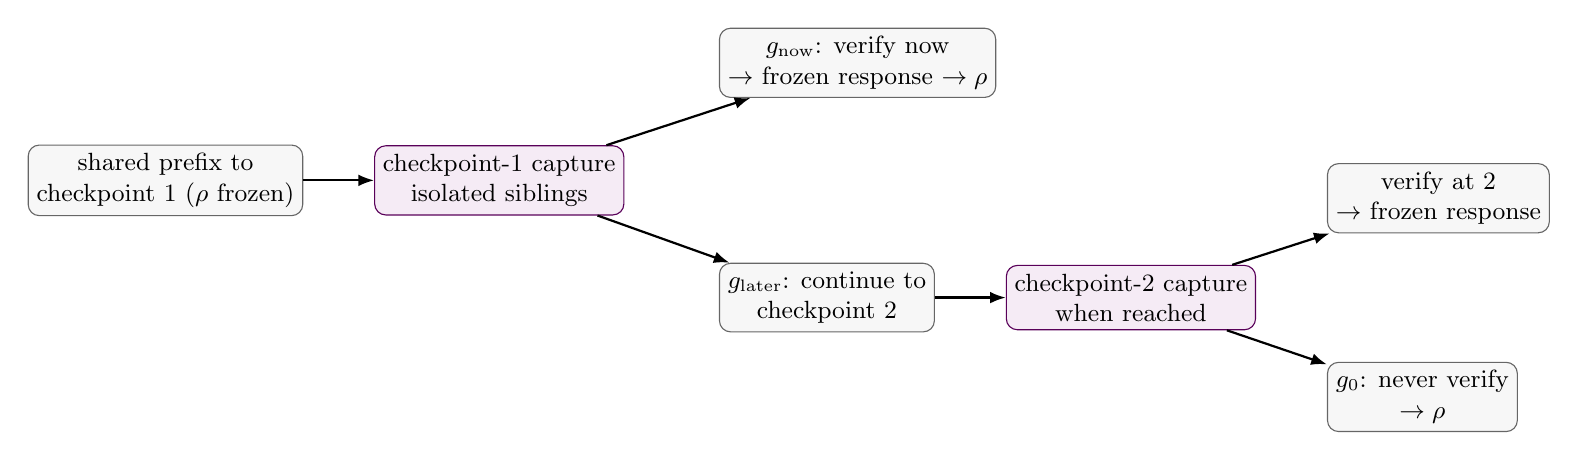
\begin{tikzpicture}[
  node distance=5mm and 9mm,
  box/.style={draw, rounded corners, align=center, inner sep=3pt, font=\small, minimum height=6.5mm},
  rnd/.style={box, draw=violet!70!black, fill=violet!8},
  fixed/.style={box, draw=black!60, fill=black!3},
  arrow/.style={-{Latex[length=2mm]}, thick}
]
\node[fixed] (prefix) {shared prefix to\\checkpoint 1 ($\rho$ frozen)};
\node[rnd, right=of prefix] (cp1) {checkpoint-1 capture\\isolated siblings};
\node[fixed, above right=6mm and 12mm of cp1] (now) {$g_{\mathrm{now}}$: verify now\\$\to$ frozen response $\to\rho$};
\node[fixed, below right=6mm and 12mm of cp1] (later) {$g_{\mathrm{later}}$: continue to\\checkpoint 2};
\node[rnd, right=of later] (cp2) {checkpoint-2 capture\\when reached};
\node[fixed, above right=4mm and 9mm of cp2] (v2) {verify at 2\\$\to$ frozen response};
\node[fixed, below right=4mm and 9mm of cp2] (never) {$g_0$: never verify\\$\to\rho$};
\draw[arrow] (prefix) -- (cp1);
\draw[arrow] (cp1) -- (now);
\draw[arrow] (cp1) -- (later);
\draw[arrow] (later) -- (cp2);
\draw[arrow] (cp2) -- (v2);
\draw[arrow] (cp2) -- (never);
\end{tikzpicture}%
}
\par\smallskip
\parbox{0.95\textwidth}{\centering\footnotesize
   At most one verifier call per root; the same frozen verifier and response rule
   are used at checkpoint 1 and checkpoint 2.  Roots that never reach
   checkpoint 2, or at which the verifier is unavailable, stay in the
   original-root analysis under the registered fallback.}
\caption{The two-checkpoint regime tree on one original root.  The prefix to
checkpoint 1 is shared; verify-now and continue fork there; the continue branch
forks again at checkpoint 2 into verify-at-2 and continue.  All original roots,
including early-terminal and infeasible ones, enter the estimand.}
\label{fig:b-architecture}
\end{figure*}

% ---------------------------------------------------------------------------
% Timing schematic: which regime is best under the declared costs, per
% mechanism class.  Schematic only; no experimental data are shown.  The
% figure records the predeclared mechanism classes and the regime ordering each
% witness must exhibit through the real adapter before any live screen.
% ---------------------------------------------------------------------------
\begin{figure}[t]
\centering
\resizebox{\linewidth}{!}{%
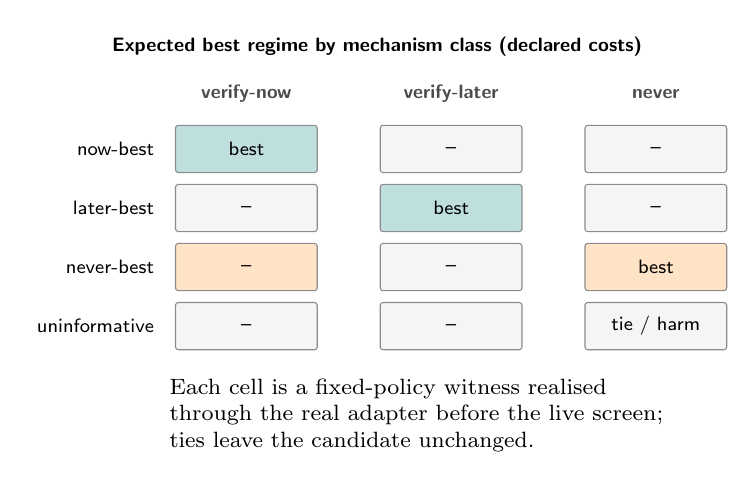
\begin{tikzpicture}[
  font=\sffamily\scriptsize,
  cell/.style={draw=black!45, rounded corners=1pt, minimum width=18mm,
               minimum height=6mm, inner sep=1pt, align=center},
  arrow/.style={-{Latex[length=1.6mm]}, line width=.5pt, black!65},
]
\node[align=center,text width=7.6cm,font=\sffamily\scriptsize\bfseries] at (1.65,2.05)
  {Expected best regime by mechanism class (declared costs)};
% header
\node[font=\sffamily\scriptsize\bfseries,text=black!70] at (0.0,1.45) {verify-now};
\node[font=\sffamily\scriptsize\bfseries,text=black!70] at (2.6,1.45) {verify-later};
\node[font=\sffamily\scriptsize\bfseries,text=black!70] at (5.2,1.45) {never};
% rows
\foreach \y/\lab in {0.75/now-best, 0.0/later-best, -0.75/never-best, -1.5/uninformative}{
  \node[anchor=east,align=right] at (-1.05,\y) {\lab};
}
\node[cell,fill=teal!25] at (0.0,0.75) {best};
\node[cell,fill=black!4] at (2.6,0.75) {--};
\node[cell,fill=black!4] at (5.2,0.75) {--};
\node[cell,fill=black!4] at (0.0,0.0) {--};
\node[cell,fill=teal!25] at (2.6,0.0) {best};
\node[cell,fill=black!4] at (5.2,0.0) {--};
\node[cell,fill=orange!22] at (0.0,-0.75) {--};
\node[cell,fill=black!4] at (2.6,-0.75) {--};
\node[cell,fill=orange!22] at (5.2,-0.75) {best};
\node[cell,fill=black!4] at (0.0,-1.5) {--};
\node[cell,fill=black!4] at (2.6,-1.5) {--};
\node[cell,fill=black!4] at (5.2,-1.5) {tie / harm};
\node[font=\footnotesize, anchor=north west, text width=6.4cm, align=left]
  at (-1.1,-2.05)
  {Each cell is a fixed-policy witness realised through the real adapter before
   the live screen; ties leave the candidate unchanged.};
\end{tikzpicture}%
}
\caption{\textbf{Timing, not ranking.}  The design asks which regime is best
under the declared costs.  Four mechanism classes are predeclared, and each is
realised by an executable fixed-policy witness through the real adapter: a world
where verifying now is best, one where reserving for checkpoint 2 is best, one
where never verifying is best, and an uninformative-or-harmful check.
\emph{Schematic: no experimental data are shown; all cells are the predeclared
target orderings, not measured outcomes.}}
\label{fig:timing}
\end{figure}


\section*{Reproducibility statement}
The prospective experimental contract is machine-readable
(\texttt{protocols/paper\_b/contract\_v2.yaml}; v1 is historical) and a launch
validator refuses to run with missing required fields.  The executable
candidate-consistency task, the \texttt{b\_branch\_v2} tree records and the
engineering smoke path (\texttt{make smoke-b}) run on CPU and report
\texttt{ENGINEERING\_ONLY}.  No scientific result is reported in this draft; the
contract's runtime, artifact, split and provenance bindings stay null until they
are bound on the substrate.

\section*{AI use statement}
Generative-AI tools assisted with editorial restructuring and software
implementation.  The authors selected the research question, protocol, formal
claims, and analysis, checked the resulting text and citations, and take
responsibility for the submission.

\bibliographystyle{icml2026}
\bibliography{references}

\newpage
\onecolumn
\appendix
\section{Proofs and equivalence checks}
\label{app:b-proofs}

This appendix contains only the proofs needed by the claims of the main text.
The inherited ordinal, abstraction and price-theoretic material that is not
needed is preserved in \texttt{papers/paper\_b/archive/B1\_20260927/}.

\subsection{The population-scoped discrepancy allowance}

\begin{proof}[Proof of \cref{prop:n1-population}]
Let $d$ be a fixed policy.  Write the signed contrast integrand
$h(W)=d(W)\,(U^v(W)-U^0(W))$, with $h(W)\in[-1,1]$ because $U\in[0,1]$ and
$d\in\{0,1\}$.  Let $D$ be the declared joint discrepancy event with
$\Prb(D)\le p$.  Off $D$ the intended and discrepancy-world regime outputs agree,
so the integrand is unchanged.  On $D$, the two regime outcomes can each move by
up to $1$, so for any $W\in D$ the integrand can change by at most $2$; the
contribution of $D$ to the population mean therefore changes by at most
$2\,\Prb(D)\le 2p$.  Combining the unchanged off-$D$ part with the bounded on-$D$
part gives
\[
 \big|\,G_{\text{discrepancy}}(d)-G(d)\,\big|\le 2p .
\]
Hence any valid lower bound $L\le G(d)$ for the intended population gain remains
valid for $G_{\text{discrepancy}}(d)$ after subtracting $2p$, i.e.\
$L-2p\le G_{\text{discrepancy}}(d)$.  The result is a population statement for a
\emph{fixed} policy; selection over a family is handled by simultaneous bounds in
the main text.
\end{proof}

\paragraph{Why the pointwise gate is not available.}
The $2p$ shift is a bound on a population mean, not on a pointwise conditional
mean.  A gate of the form $\mathrm{LCB}(w)-2p>0$ applied per checkpoint would
require a conditional allowance that is not implied by the global event; the
main text therefore forbids it and uses simultaneous population bounds for
family selection.

\subsection{Ridge advantage/action-value equivalence}
\label{app:b-ridge}

Let $B$ be the common ridge fitting operator on paired rows, with identical
design matrices, penalties and rows for the advantage learner and the
action-value learner.  Ridge is affine in the response and the two learners share
the same design matrix, so
\[
 \widehat{\text{adv}} = B\,(y_v-y_0)=B\,y_v-B\,y_0
 = \widehat{q}_v-\widehat{q}_0 ,
\]
up to floating-point error.  On identical designs the two estimators must agree
to within $10^{-12}$; this is an implementation equivalence check, not a
hypothesis and not a contribution.

\subsection{Corrected conditional-expectation statement}
\label{app:b-conditional}

An earlier inherited version of this appendix asserted that, with
cell-measurable policies, the integrand equals the cell-level advantage of the
regime selected in its cell, so that cell-level validity applies
\emph{pointwise}.  That pointwise equality does not hold in general: the
integrand is a random function whose realised value depends on the within-cell
state, whereas the cell-level advantage is a conditional mean.  What holds is
only the \emph{conditional-expectation} identity
\[
 \E\!\left[\,\Delta^{(j)}_{d(Z,M)}(Z,M)\ \middle|\ c(Z,M)\,\right]
 = \Delta^{(j)}_{\text{selected at }c(Z,M)}\big(c(Z,M)\big),
\]
because conditioning on the cell fixes the selected regime.  Cell-level validity
therefore transfers through the conditional expectation, not through a pointwise
equality.  This corrects the inherited assertion.


\end{document}
